\chapter{Конструкторская часть}
\label{cha:design}

\section{Требования к программе}

Программа должна предоставлять следующие возможности.

\begin{enumerate}
	\item Визуализацию сцены.
	\item Запуск системы.
	\item Останов системы.
\end{enumerate}

\section{Алгоритм обратной трассировки лучей}

В данном проекте алгоритм обратной трассировки лучей будет применяться к сфере и цилиндру.
Для того, чтобы воспользоваться данным алгоритмом, нужно уметь находить пересечение луча со сферой и цилиндром.

\subsection {Пересечения луча и сферы}

Уравнение луча представлено ниже:

\begin{equation}
	P = O + t(V - O), t \geq 0,
	\label{eq:ref5}
\end{equation}
где О - центр камеры, а V - текущий пиксель.

Обозначим направление луча:

\begin{equation}
	\overrightarrow{D} = V - O
\end{equation}

Уравнение \eqref{eq:ref5_1} эквивалентно уравнению \eqref{eq:ref5}

\begin{equation}
	{\begin{cases}
			x(t) = x_O + t x_D \\
			y(t) = y_O + t y_D \\
			z(t) = z_O + t z_D
			\label{eq:ref5_1}
		\end{cases}}
\end{equation}

Рассмотрим, что собой представляет сфера.

%\begin{figure}[ht!]
%	\centering{
%		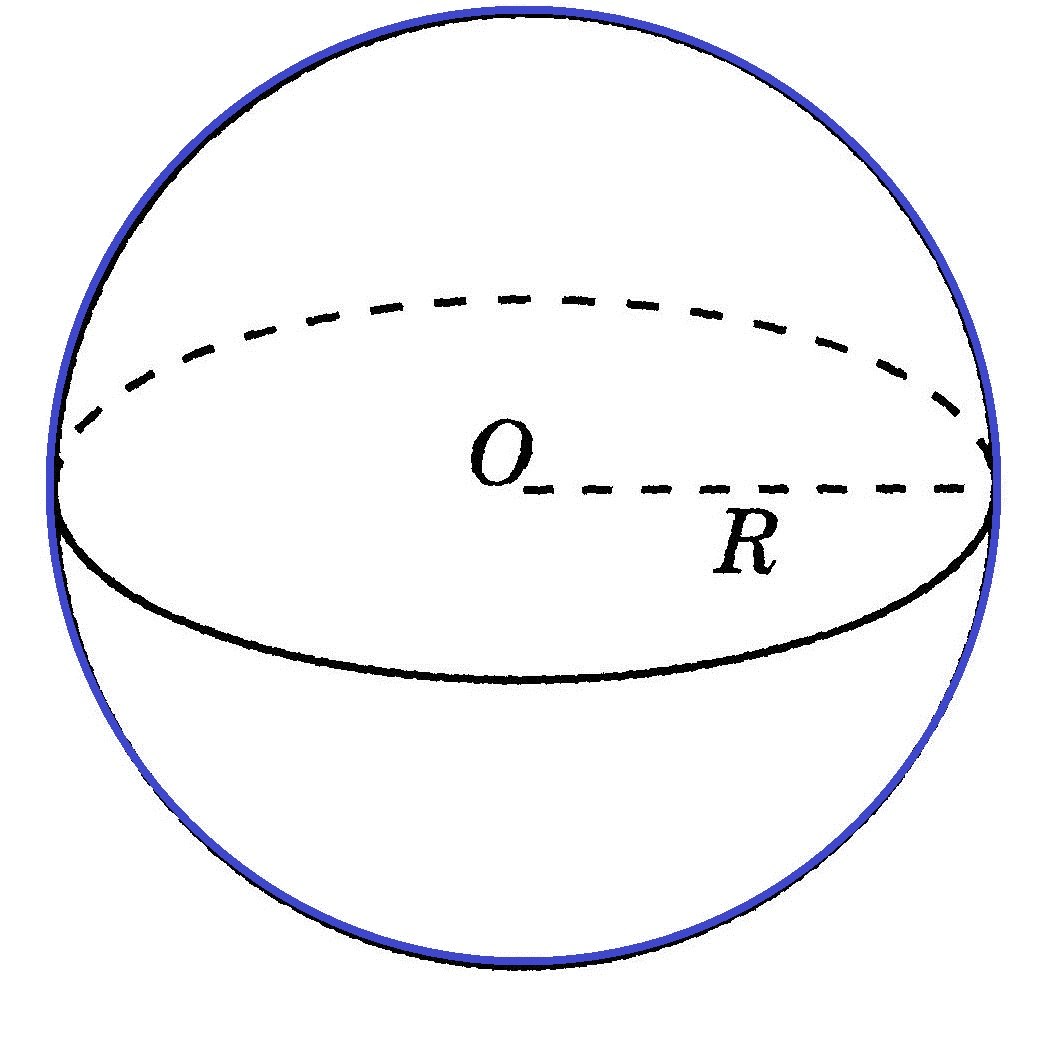
\includegraphics[width=0.5\textwidth]{img/sphere.jpg}
%		\caption{Сфера}}
%\end{figure}

Сфера — это множество точек P, лежащих на постоянном расстоянии r от фиксированной точки C. Тогда можно записать уравнение, удовлетворяющее этому условию:

\begin{equation}
	distance(P,C) = r
	\label{eq:ref6}
\end{equation}

Запишем расстояние (\ref{eq:ref6}) между P и C как длину вектора из P в C.

\begin{equation}
	|P-C|=r
\end{equation}

Заменим на скалярное произведение вектора на себя:

\begin{equation}
	\sqrt{\langle P - C\rangle, \langle P - C\rangle} = r
\end{equation}

Избавимся от корня:

\begin{equation}
	\langle P - C\rangle, \langle P - C\rangle = r^2
	\label{eq:ref7}
\end{equation}

В итоге есть два уравнения - уравнение луча и сферы. Найдем пересечение луча со сферой. Для этого подставим (\ref{eq:ref5}) в (\ref{eq:ref7})

\begin{equation}
	\langle O + t\overrightarrow{D} - C \rangle, \langle O + t\overrightarrow{D} - C\rangle = r^2
\end{equation}

Разложим скалярное произведение и преобразуем его. В результате получим:

\begin{equation}
	t^2 \langle \overrightarrow{D}, \overrightarrow{D} \rangle + 2t \langle \overrightarrow{OC}, \overrightarrow{D} \rangle + \langle \overrightarrow{OC}, \overrightarrow{OC} \rangle -r^2 = 0
	\label{eq:ref8}
\end{equation}

Представленное квадратное уравнение (\ref{eq:ref8}) имеет несколько возможнных случаев решения.
Если у уравнения одно решение, это обозначает, что луч касается сферы.
Два решения обозначают, то что луч входит в сферу и выходит из неё.
И если нет решений, значит, луч не пересекается со сферой.

\subsection {Пересечения луча и цилиндра}

Бесконечный цилиндр, образующие которого параллельны оси z, описывается уравнением\eqref{eq:ref9}

\begin{equation}
	x^2 + y^2 = r^2
	\label{eq:ref9}
\end{equation}

Аналогичные уравнения \eqref{eq:ref10} и \eqref{eq:ref11} для
бесконечных цилиндров, образующие которых параллельны осям x и y соответственно.

\begin{equation}
	y^2 + z^2 = r^2
	\label{eq:ref10}
\end{equation}

\begin{equation}
	x^2 + z^2 = r^2
	\label{eq:ref11}
\end{equation}

Рассмотрим цилиндр, выровненный вдоль оси z (уравнение \ref{eq:ref9}).
Аналогичные решения получатся для \eqref{eq:ref10} и \eqref{eq:ref11}.
Найдем пересечение луча с цилиндром.
Для этого подставим \eqref{eq:ref5_1} в \eqref{eq:ref9}

\begin{equation}
	(x_O + t x_D)^2 + (y_O + t y_D)^2 = r^2
	\label{eq:ref12}
\end{equation}

Вынесем t из скобок в уравнение \eqref{eq:ref12} и получим \eqref{eq:ref13}

\begin{equation}
	t^2(x_D^2+y_D^2) + 2t(x_Ox_D + y_Oy_D) + (x_O^2 + y_O^2 - r^2) = 0
	\label{eq:ref13}
\end{equation}

Решение представленного уравнения (\ref{eq:ref13}) можно получить решив дискриминант.
Уравнение (\ref{eq:ref13}) квадратное и имеет соответствующие случаи решения.


Для конечного цилиндра нужно ввести ограничение по оси.
Для цилиндра, записанного уравнением (\ref{eq:ref9}), данные ограничения
продемонстрированы в (\ref{eq:ref14})

\begin{equation}
	z_{min} < z < z_{max}
	\label{eq:ref14}
\end{equation}

Получив $t_1$ и $t_2$ из уравнения (\ref{eq:ref13})
найдем $z_1$ и $z_2$ с помощью уравнения (\ref{eq:ref5_1}).
Далее необходимо произвести проверку (\ref{eq:ref15})

\begin{equation}
	{\begin{cases}
			z_{min} < z_1 < z_{max} \\
			z_{min} < z_2 < z_{max}
			\label{eq:ref15}
		\end{cases}}
\end{equation}

Если обе точки проходят данный тест, то наименьшее неотрицательное
значение t -- это ближайшая точка пересечения луча с конечным цилиндром.

\subsection {Алгоритм трассировки лучей}

Суть алгоритма состоит в следующем.

Из некоторой точки пространства, называемой виртуальным глазом, или камерой,
через каждый пиксель изображения испускается луч и находится
точка пересечения с объектом сцены (\ref{eq:ref8} и \ref{eq:ref13}).
Далее из найденной точки пересечения испускаются лучи до каждого источника освещения.
Если данные лучи пересекают другие объекты сцены, значит точка пересечения находится
в тени относительно рассматриваемого источника освещения и освещать ее не нужно.
Освещение со всех видимых источников света складываются  (по интенсивности).
Далее, если материал рассматриваемого объекта имеет отражающие или преломляющие свойства, из точки
испускается отраженный луч, и для него вся процедура трассировки рекурсивно повторяется.

На рис. \eqref{fig:ref3} представлена схема алгоритма.

\begin{figure}[ht!]
	\centering{
		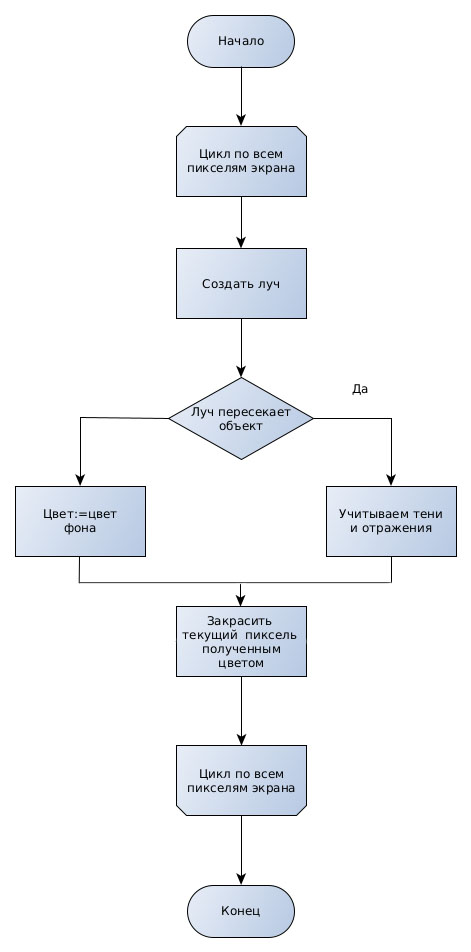
\includegraphics[width=0.5\textwidth]{block_diagram.jpg}
		\caption{Cхема алгоритма трассировки лучей}
		\label{fig:ref3}}
\end{figure}

\section{Выбор используемых типов и структур данных}

В данной работе нужно будет реализовать следующие типы и структуры данных.

\begin{enumerate}
	\item Точка -- хранит положение, задается координатами x, y, z.
	\item Вектор -- хранит направление, задается x, y, z.
	\item Цвет -- вектор из трех чисел (синий, красный, зеленый).
	\item Сфера -- хранит радиус, цвет и центр сферы.
	\item Цилиндр -- хранит радиус, цвет, центр цилиндра и ось (x, y или z), образующие цилиндра параллельны ей.
	\item Сцена -- список объектов, заданных сферами и цилиндрами.
	\item Источник света -- положение и направление света.
\end{enumerate}

\section {Уменьшение времени работы трассировки лучей}

Параллельные вычисления часто используются для уменьшения времени работы алгоритмов.

Поскольку алгоритм обратной трассировки лучей обрабатывает каж-
дый пиксель экрана независимо, можно распараллелить обработку всего
экрана, разбив его на некоторые части.
Разбиение экрана можно производить горизонтально или вертикально.
После разбиения каждый поток будет обрабатывать свой участок экрана.

На рис. \eqref{ref:rimg1} показано, как можно вертикально разбить экран на
несколько частей. На рис. \eqref{ref:rimg2} показано горизонтальное разбиение экрана.
Разбив экран на части можно реализовывать параллельное вычисление цвета
пикселей каждой части экрана.

\begin{figure}[ht!]
	\centering{
		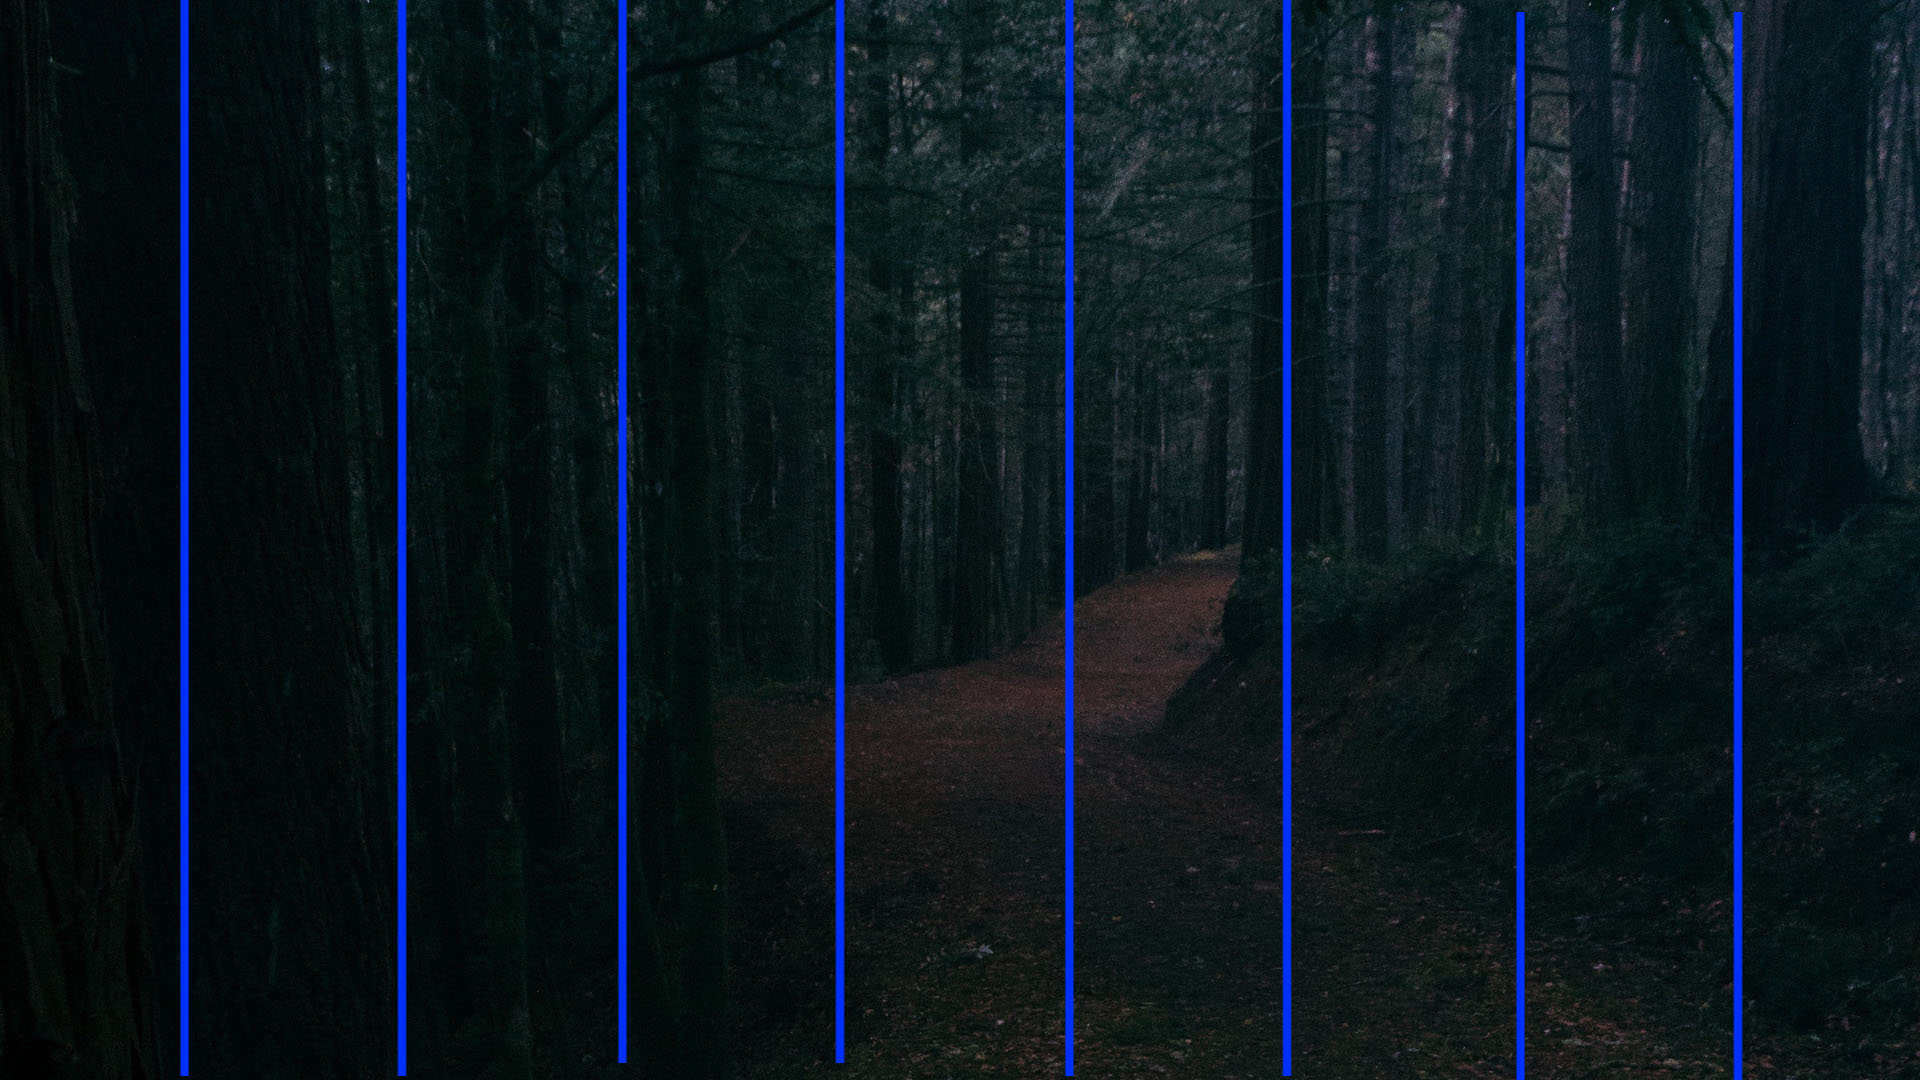
\includegraphics[width=0.8\textwidth]{h.jpg}
		\caption{Вертикальное разбиение экрана}
		\label{ref:rimg1}}
\end{figure}

\begin{figure}[ht!]
	\centering{
		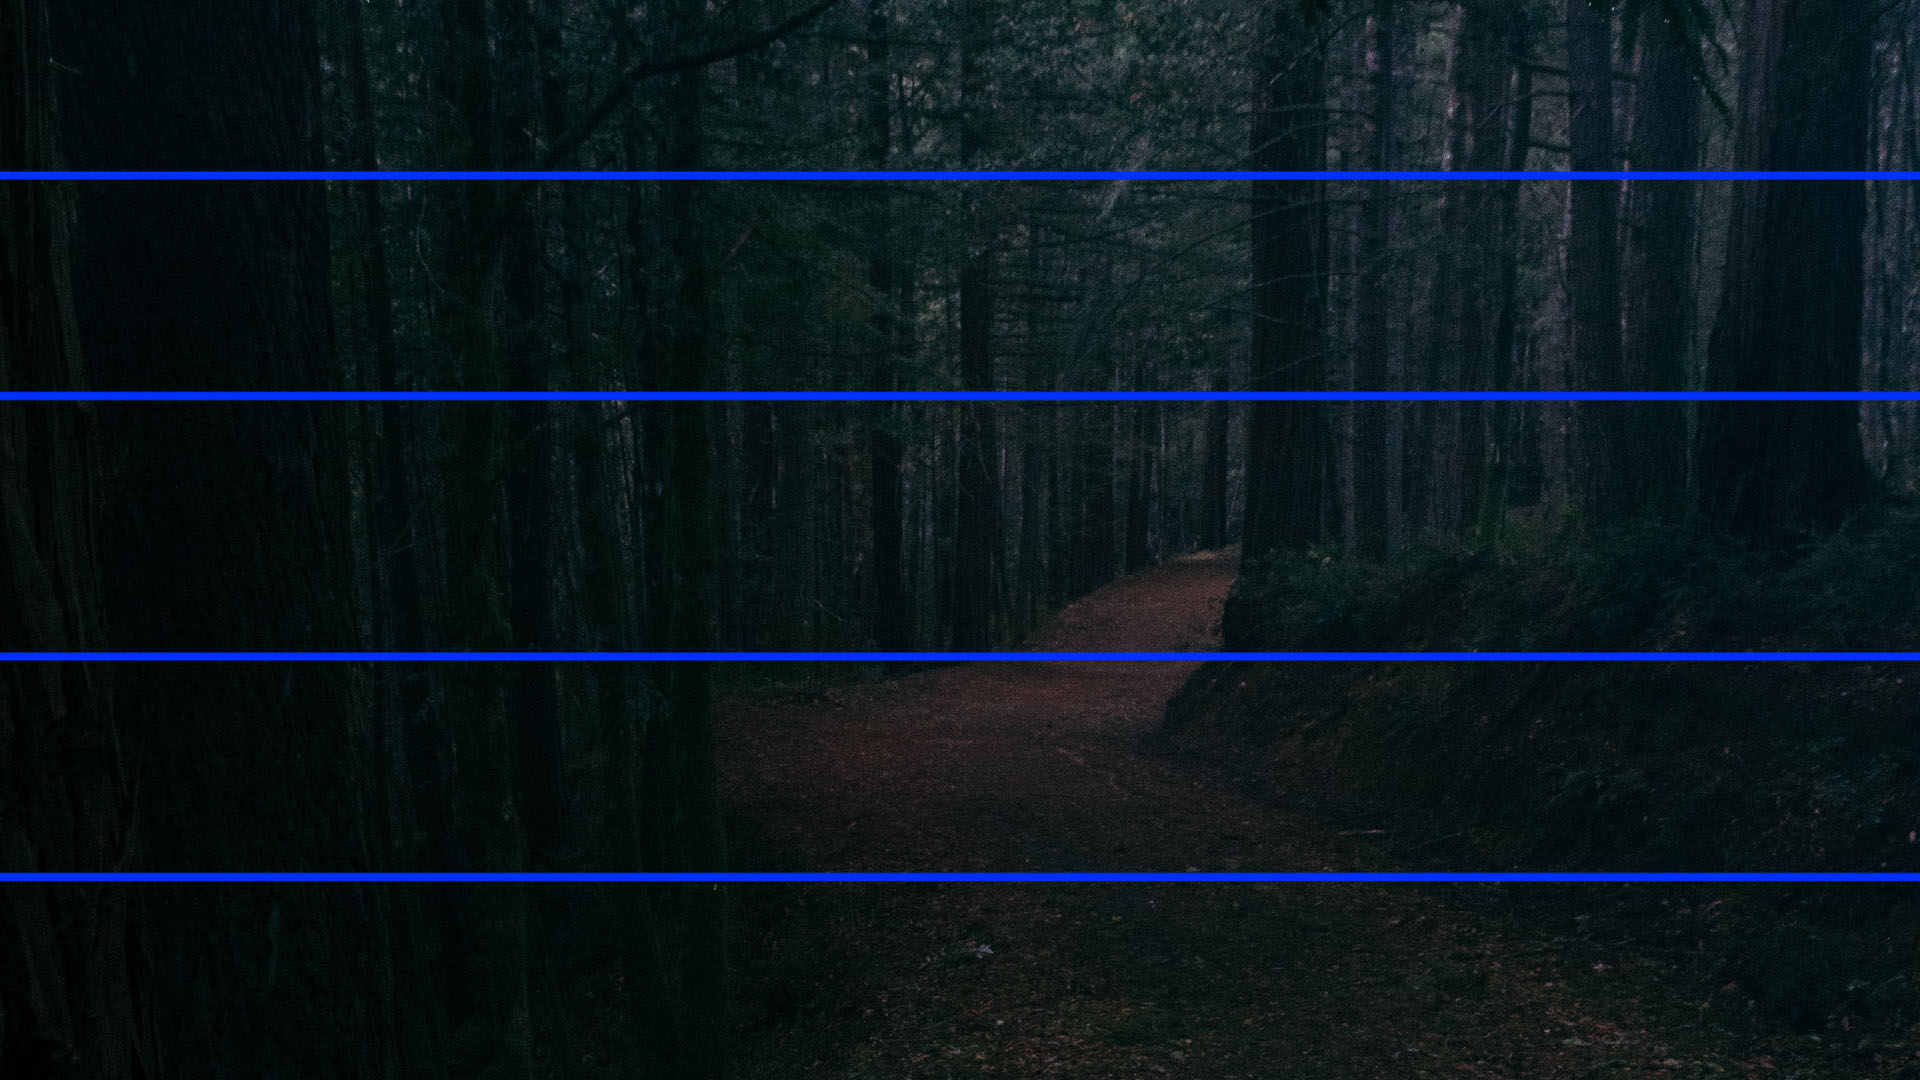
\includegraphics[width=0.8\textwidth]{w.jpg}
		\caption{Горизонтальное разбиение экрана}
		\label{ref:rimg2}}
\end{figure}

\section{Вывод}

В данном разделе были описаны требования к программе, подробно рассмотрен алгоритм трассировки лучей,
описаны типы и структуры данных, которые будут реализованы,
и приведена схема алгоритма трассировки лучей.
Также рассмотрено многопоточное выполнение которое будет применено в данном проекте для уменьшения времени работы алгоритма.
